\documentclass[border=5pt]{standalone}
\usepackage{tikz}
\usetikzlibrary{shapes,arrows.meta,positioning,backgrounds,fit,calc,decorations.pathreplacing,shadows}
\usepackage{amsmath,amssymb}
\usepackage{xcolor}

% Colour palette — matched to pam-architecture.tex
\definecolor{wp1col}{RGB}{66,133,244}     % blue — memory
\definecolor{wp2col}{RGB}{171,71,188}     % purple — reasoning
\definecolor{wp3col}{RGB}{38,166,154}     % teal — environments
\definecolor{memcol}{RGB}{171,71,188}     % purple
\definecolor{hdccol}{RGB}{255,167,38}     % orange — HDC
\definecolor{errcol}{RGB}{229,57,53}      % red — prediction error
\definecolor{bglight}{RGB}{248,248,252}
\definecolor{arrowgray}{RGB}{120,120,140}

\begin{document}
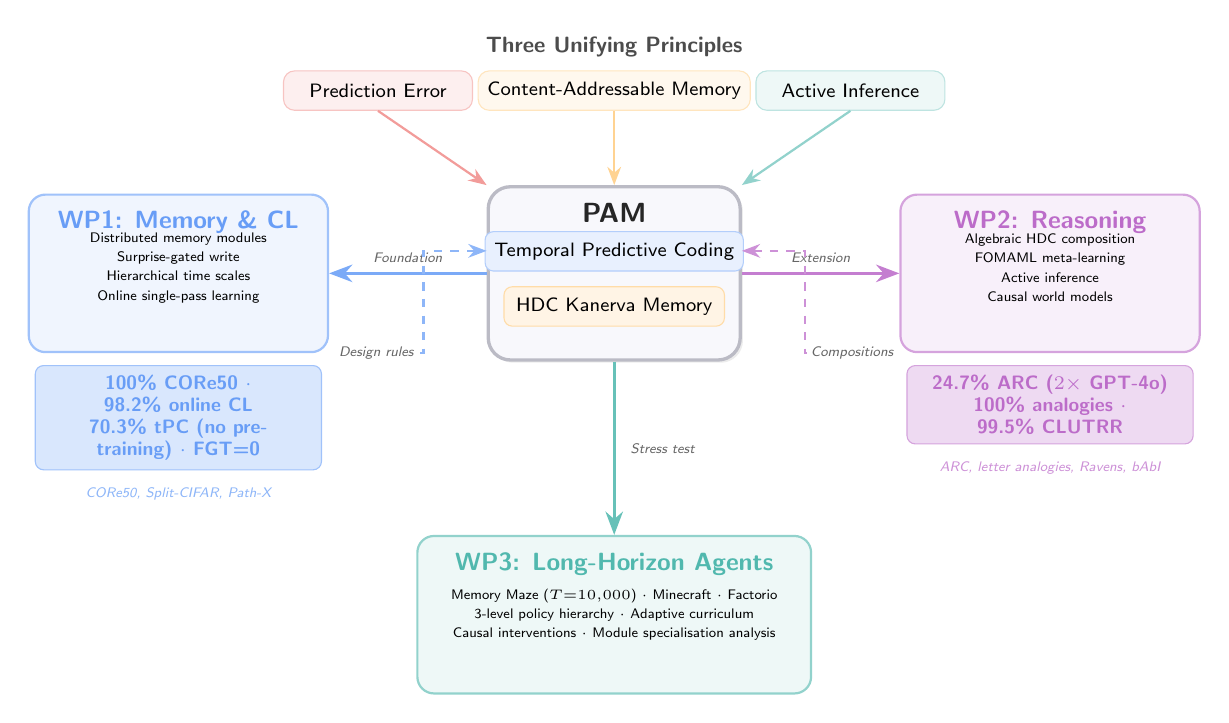
\begin{tikzpicture}[
    >=Stealth,
    node distance=0.5cm and 0.7cm,
    wpbox/.style={draw, rounded corners=6pt, minimum height=2.0cm, minimum width=3.8cm,
                  font=\small\sffamily, thick, fill=#1!8, draw=#1!50},
    resultbox/.style={draw, rounded corners=3pt, minimum height=0.4cm,
                      font=\scriptsize\sffamily\bfseries, fill=#1!20, draw=#1!50, text=#1!80},
    mechbox/.style={draw, rounded corners=3pt, minimum height=0.5cm, minimum width=2.8cm,
                    font=\scriptsize\sffamily, fill=#1!12, draw=#1!40},
    arr/.style={->, thick, color=arrowgray},
    darr/.style={->, thick, dashed, color=#1!60},
    biglabel/.style={font=\small\sffamily\bfseries, color=#1!80},
    label/.style={font=\tiny\sffamily\itshape, color=black!60},
]

% ============ CENTRAL PAM CORE ============
\node[draw, rounded corners=8pt, minimum height=2.2cm, minimum width=3.2cm,
      fill=bglight, draw=arrowgray!50, very thick, drop shadow={shadow xshift=1pt, shadow yshift=-1pt, opacity=0.15}]
      (pam) {};
\node[font=\normalsize\sffamily\bfseries, color=black!85] at (pam.north) [anchor=north, yshift=-3pt] {PAM};

% PAM internal components
\node[mechbox=wp1col, yshift=-2pt] at ($(pam.center) + (0, 0.35)$) (tpc) {Temporal Predictive Coding};
\node[mechbox=hdccol, yshift=-2pt] at ($(pam.center) + (0, -0.35)$) (hdc) {HDC Kanerva Memory};

% ============ WP1: MEMORY & CL (LEFT) ============
\node[wpbox=wp1col, left=2.0cm of pam] (wp1) {};
\node[biglabel=wp1col] at (wp1.north) [anchor=north, yshift=-3pt] {WP1: Memory \& CL};

% WP1 content
\node[font=\tiny\sffamily, text width=3.2cm, align=center] at (wp1.center) [yshift=2pt] {
    Distributed memory modules\\[1pt]
    Surprise-gated write\\[1pt]
    Hierarchical time scales\\[1pt]
    Online single-pass learning
};

% WP1 results
\node[resultbox=wp1col, below=0.15cm of wp1.south, text width=3.4cm, align=center] (wp1r) {
    100\% CORe50 $\cdot$ 98.2\% online CL\\
    70.3\% tPC (no pretraining) $\cdot$ FGT=0
};

% ============ WP2: COMPOSITIONAL REASONING (RIGHT) ============
\node[wpbox=wp2col, right=2.0cm of pam] (wp2) {};
\node[biglabel=wp2col] at (wp2.north) [anchor=north, yshift=-3pt] {WP2: Reasoning};

% WP2 content
\node[font=\tiny\sffamily, text width=3.2cm, align=center] at (wp2.center) [yshift=2pt] {
    Algebraic HDC composition\\[1pt]
    FOMAML meta-learning\\[1pt]
    Active inference\\[1pt]
    Causal world models
};

% WP2 results
\node[resultbox=wp2col, below=0.15cm of wp2.south, text width=3.4cm, align=center] (wp2r) {
    24.7\% ARC ($2{\times}$ GPT-4o)\\
    100\% analogies $\cdot$ 99.5\% CLUTRR
};

% ============ WP3: ENVIRONMENTS (BOTTOM) ============
\node[wpbox=wp3col, below=2.2cm of pam, minimum width=5.0cm] (wp3) {};
\node[biglabel=wp3col] at (wp3.north) [anchor=north, yshift=-3pt] {WP3: Long-Horizon Agents};

\node[font=\tiny\sffamily, text width=4.5cm, align=center] at (wp3.center) [yshift=0pt] {
    Memory Maze ($T{=}10{,}000$) $\cdot$ Minecraft $\cdot$ Factorio\\[1pt]
    3-level policy hierarchy $\cdot$ Adaptive curriculum\\[1pt]
    Causal interventions $\cdot$ Module specialisation analysis
};

% ============ ARROWS: PAM <-> WPs ============
\draw[arr, wp1col!70, line width=1.2pt] (pam.west) -- node[above, label] {Foundation} (wp1.east);
\draw[arr, wp2col!70, line width=1.2pt] (pam.east) -- node[above, label] {Extension} (wp2.west);
\draw[arr, wp3col!70, line width=1.2pt] (pam.south) -- node[right, label, xshift=2pt] {Stress test} (wp3.north);

% Feedback arrows (labels on-path, white-filled so they anchor to their arrow)
\draw[darr=wp1col, <-] (pam.170) -- ++(-0.8,0) |- node[pos=0.75, label, fill=white, inner sep=1.5pt] {Design rules} (wp1.east |- wp1.south east);
\draw[darr=wp2col, <-] (pam.10) -- ++(0.8,0) |- node[pos=0.75, label, fill=white, inner sep=1.5pt] {Compositions} (wp2.west |- wp2.south west);

% ============ TOP: THREE PRINCIPLES ============
\node[draw, rounded corners=4pt, fill=errcol!8, draw=errcol!30, minimum height=0.5cm, minimum width=2.4cm,
      font=\scriptsize\sffamily] at ($(pam.north) + (-3.0, 1.2)$) (p1) {Prediction Error};
\node[draw, rounded corners=4pt, fill=hdccol!8, draw=hdccol!30, minimum height=0.5cm, minimum width=2.4cm,
      font=\scriptsize\sffamily] at ($(pam.north) + (0, 1.2)$) (p2) {Content-Addressable Memory};
\node[draw, rounded corners=4pt, fill=wp3col!8, draw=wp3col!30, minimum height=0.5cm, minimum width=2.4cm,
      font=\scriptsize\sffamily] at ($(pam.north) + (3.0, 1.2)$) (p3) {Active Inference};

\draw[arr, errcol!50] (p1.south) -- (pam.north west);
\draw[arr, hdccol!50] (p2.south) -- (pam.north);
\draw[arr, wp3col!50] (p3.south) -- (pam.north east);

% Title above principles
\node[font=\footnotesize\sffamily\bfseries, color=black!70] at ($(p2.north) + (0, 0.3)$) {Three Unifying Principles};

% ============ BOTTOM LABELS: Benchmarks ============
\node[font=\tiny\sffamily\itshape, color=wp1col!60, anchor=north] at ($(wp1r.south) + (0, -0.1)$) {CORe50, Split-CIFAR, Path-X};
\node[font=\tiny\sffamily\itshape, color=wp2col!60, anchor=north] at ($(wp2r.south) + (0, -0.1)$) {ARC, letter analogies, Ravens, bAbI};

\end{tikzpicture}
\end{document}
